%!TEX root = ../../../memoria.tex
\section{Profile}

La \uiSiglaAS de profile permite ver y editar información relacionada directamente con el usuario. Esta información esta dividida en tres partes: actualización de contraseña, ordenes, y libreta de direcciones.

\subsubsection{Actualizar contraseña}

El formulario de actualización de contraseña permite al usuario cambiar tanto como desee la contraseña que tiene actualmente. Despues de todo el cambio periodico de una contraseña es una medida de seguridad básica \cite{zviran1999password}.
%The periodic changing ofa password is a basic security measure  

Como se puede observa en la \refFigura{figure:profile:form:form_update_password}, el formulario de atualización de contraseña cuenta con dos campos obligatorios para el proceso. El primero corresponde al campo de solicitud de contraseña actual (a modo de confirmación de que la persona que esta actualizando la contraseña, sea el dueño de la cuenta) y el segundo campo, para ingresar la nueva contraseña. Al apretar el botón de confirmación esta se cambia.

\begin{figure}[H]
	\centering
	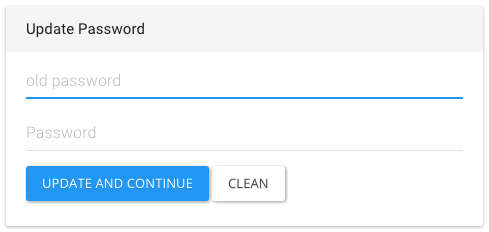
\includegraphics[width=0.5\textwidth]{figuras/profile/form_update_password.png}

	\caption{Formulario de actualización de contraseña.}
	\label{figure:profile:form:form_update_password}
\end{figure}

Existen diversas situaciones en donde el formulario notifica sobre errores que se comenten  al momento de llenar el formulario. Por ejemplo, al intentar enviar el formulario sin información ambos campos tienen errores y pueden observarse en la \refFigura{figure:profile:form:update_password:empty_form_send}.



\begin{table}[H]
    \centering
	\begin{tabular}{ |l|c||l| }
		\hline Campo & Requerido & Restricción \\ \hline
		\multirow{1}{*}{\textit{Current Password}} 	&  \checkmark 					&  Debe ser la contraseña actual\\ \hline
		\multirow{2}{*}{\textit{Password}} 			&  \multirow{2}{*}{\checkmark}	&  - Debe tener al menos  caracteres.\\
													&  								&  - Debe tener al menos un número ó símbolo.\\ \hline
	\end{tabular}
 	\caption{Resumen restrincciones formulario edición de contraseña (\refFigura{figure:apendice:profile:form:update_password:empty_form_send}  y \refFigura{figure:apendice:profile:form:update_password:week_password}).}
    \label{tab:profile:form:restrictions:update_password}
\end{table}


Tanto en la \refFigura{figure:apendice:profile:form:update_password:empty_form_send} y en la \refFigura{figure:apendice:profile:form:update_password:week_password} se puede observar que la nueva contraseña no cumple con estos requerimientos.
Los requerimientos solicitados no responden a ninguna política de seguridad actual. Simplemente se eligieron esos requerimientos para evitar contraseñas aún más débiles que las que se pueden generar.


Existe un último error, y corresponde simplemente cuando el usuario no logra identificarse correctamente, o lo que es equivalente, la contraseña actual ingresada no es correcta. En la \refFigura{figure:apendice:profile:form:update_password:incorrect_password} puede observarse el mensaje que el formulario entrega en este caso.


% \subsubsection{Ordenes de compra}

% 	El backend de las ordenes de compra aún no esta terminado, de momento solo esta el mensaje cuando no hay ninguna orden (\refFigura{figure:profile:orders_empty}).

% 	\begin{figure}[H]
% 	\centering
% 	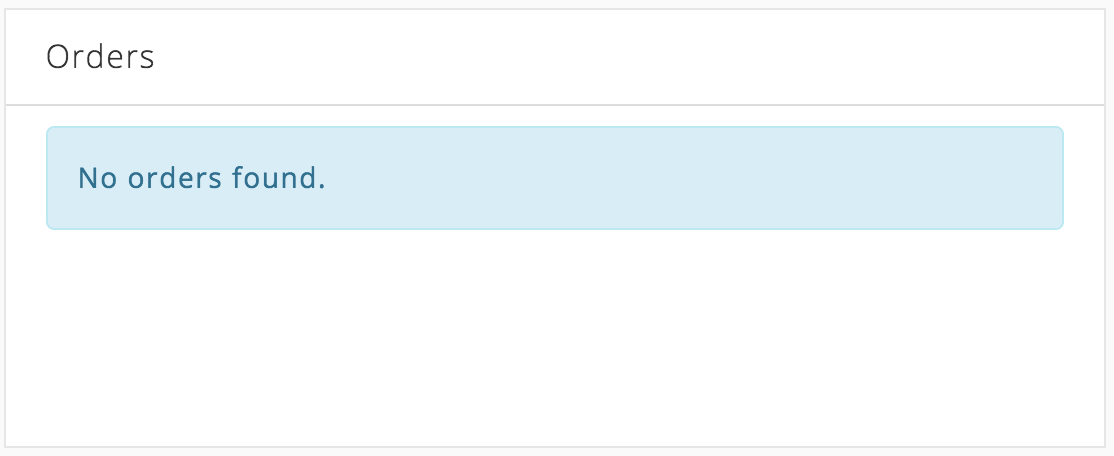
\includegraphics[width=0.5\textwidth]{figuras/profile/orders_empty.png}

% 	\caption{Vista de ordenes cuando no hay ninguna.}
% 	\label{figure:profile:orders_empty}
% \end{figure}



\subsubsection{Libreta de direcciones}

Corresponde a todas las direcciones que el usuario a agregado al sistema con el fín de utilizarlas para la recepción del o los productos. Cada uno de los parámetros del formulario para una dirección, fueron elegidos a partir del formulario de direcciónes que utiliza \amazonNAME (\refFigura{figure:apendice:address:example:amazon_address}).

\begin{table}[H]
    \centering
	\begin{tabular}{ |l|c||l| }
		\hline Campo & Requerido & Restricción \\ \hline
		\multirow{1}{*}{\textit{Country}} 			&  \checkmark 	&  Debe ser uno de las alternativas\\ \hline
		\multirow{1}{*}{\textit{Full Name}} 		&  \checkmark	& \\ \hline
		\multirow{1}{*}{\textit{Address 1}} 		&  \checkmark	& \\ \hline
		\multirow{1}{*}{\textit{Address 2}} 		&  				& \\ \hline
		\multirow{1}{*}{\textit{Postal}} 			&  \checkmark	& \\ \hline
		\multirow{1}{*}{\textit{City}} 				&  \checkmark	& \\ \hline
		\multirow{1}{*}{\textit{Region}} 			&  \checkmark	& Para ciertos paises, existen alternativas definidas.\\ \hline
		\multirow{1}{*}{\textit{Phone}} 			&  \checkmark	& \\ \hline
		\multirow{1}{*}{\textit{Shipping address}} 	&  \checkmark	& Boolean \\ \hline
		\multirow{1}{*}{\textit{billing address}} 	&  \checkmark	& Boolean \\ \hline
		\multirow{1}{*}{\textit{comercial address}} &  \checkmark	& Boolean \\ \hline
	\end{tabular}
 	\caption{Resumen restrincciones formulario para libreta de direcciones.}
    \label{tab:profile:form:restrictions:address}
\end{table}

